\documentclass[a4paper]{article}
\usepackage[italian]{babel}
\usepackage[style=ieee,backend=biber]{biblatex} \addbibresource{bibliography.bib}
\usepackage{csquotes}
\usepackage{hyperref}
\usepackage{algorithm}
\usepackage{algpseudocode}
\usepackage[table]{xcolor}
\usepackage{minted}
\usepackage{amsmath}
\usepackage{listings}
\usepackage{xcolor}
\usepackage{graphicx}
\usepackage{hyperref}
\usepackage{amssymb}
\DeclareMathOperator{\lcm}{lcm}

\lstset{
    language=C++,
    basicstyle=\ttfamily\small,
    keywordstyle=\color{blue},
    commentstyle=\color{gray},
    stringstyle=\color{red},
    numbers=left,
    numberstyle=\tiny\color{gray},
    stepnumber=1,
    numbersep=10pt,
    tabsize=2,
    showspaces=false,
    showstringspaces=false,
    breaklines=true,
    frame=single,
    backgroundcolor=\color{lightgray},
    captionpos=b
}

\title{Report PHPC}
\author{Pierluigi Supino \and Rodolfo Diana \and Salvatore Di Gennaro}

\begin{document}

\maketitle
\tableofcontents

\section{Introduzione}

Sviluppare un’applicazione per il prodotto tra matrici su cluster multi-nodo e multi-GPU per nodo (MPI + CUDA, attraverso SLURM).

Definiamo formalmente l'operazione di prodotto tra matrici.
Siano date una matrice $\mathbf{A} \in \mathbb{R}^{m\times{k}}$ ed una seconda matrice $\mathbf{B} \in \mathbb{R}^{k\times{n}}$.
Si definisce il prodotto matriciale di $\mathbf{A}$ per $\mathbf{B}$ la matrice $\mathbf{C}=\mathbf{A}\mathbf{B} \in \mathbb{R}^{m\times{n}}$ in cui ogni elemento $\mathbf{C}_{i,j}$ è dato dal prodotto scalare tra la $i$-esima riga di $\mathbf{A}$ per la $j$-esima colonna di $\mathbf{B}$:
$$ \mathbf{C}_{i,j} = \sum_{l=0}^{\text{k}-1} \mathbf{A}_{i, l} \mathbf{B}_{l, j} $$

\section{Implementazione}
In un ambiente multi-nodo e multi-GPU, il prodotto tra matrici può essere articolato in due livelli distinti ma interconnessi.

A un livello più alto è necessario decomporre il problema a livello globale, ovvero suddividere le matrici da moltiplicare in blocchi che possano essere assegnati in modo efficiente ai diversi nodi del cluster, tenendo conto del bilanciamento del carico, della minimizzazione della comunicazione tra nodi e dell'architettura del sistema.

A un livello più basso, invece, entra in gioco l’effettiva esecuzione del prodotto tra i blocchi locali di matrici all’interno di ciascun nodo, sfruttando le GPU a disposizione. Si potrebbe ulteriormente suddividere questo livello in partizionamento delle matrice tra le diverse GPU ed esecuzione dei calcoli.

\subsection{Processi}
Esistono numerosi modi di eseguire un prodotto matriciale in maniera distribuita. In questo contesto è stato deciso di implementarlo tramite SUMMA (Scalable Universal Matrix Multiplication Algorithm), un algoritmo efficiente e scalabile in ambiente multi-nodo\cite{SUMMA}.

Supponiamo di disporre i diversi processi partecipanti in una griglia logica bidimensionale $r \times c$ e sia $l=\lcm(r, c)$. È possibile suddividere le matrici nel seguente modo:
$$
    \mathbf{A}=
    \begin{bmatrix}
        \mathbf{A}^{0,0}     & \cdots & \mathbf{A}^{0,(l-1)}     \\
        \vdots               & \ddots & \vdots                   \\
        \mathbf{A}^{(r-1),0} & \cdots & \mathbf{A}^{(r-1),(l-1)}
    \end{bmatrix}
$$

$$
    \mathbf{B}=
    \begin{bmatrix}
        \mathbf{B}^{0,0}     & \cdots & \mathbf{B}^{0,(c-1)}     \\
        \vdots               & \ddots & \vdots                   \\
        \mathbf{B}^{(l-1),0} & \cdots & \mathbf{B}^{(l-1),(c-1)}
    \end{bmatrix}
$$

$$
    \mathbf{C}=
    \begin{bmatrix}
        \sum_{k=0}^{l-1}\mathbf{A}^{0,k}\mathbf{B}^{k,0}     & \cdots & \sum_{k=0}^{l-1}\mathbf{A}^{0,k}\mathbf{B}^{k,(c-1)}     \\
        \vdots                                               & \ddots & \vdots                                                   \\
        \sum_{k=0}^{l-1}\mathbf{A}^{(r-1),k}\mathbf{B}^{k,0} & \cdots & \sum_{k=0}^{l-1}\mathbf{A}^{(r-1),k}\mathbf{B}^{k,(c-1)}
    \end{bmatrix}
$$

Ad ogni processo $P_{i,j}$ vengono assegnati i blocchi $\mathbf{A}^{i,s}$ per cui $\bmod(s,l)=j$, e i blocchi $\mathbf{B}^{t,j}$ per cui $\bmod(t,l)=i$.
L'algoritmo si svolge in più passaggi nei quali i processi collaborano per combinare blocchi specifici. Ad ogni passo $k$, il processo che possiede il blocco $\mathbf{A}^{i,k}$ lo invia alla propria riga e, analogamente, il possessore del blocco $\mathbf{B}^{k,j}$ alla propria colonna.
Una volta ricevuti i blocchi necessari, ogni processo può calcolare una parte del prodotto parziale della matrice $\mathbf{C}$, sommando il risultato a quello già accumulato. Ripetendo questa operazione, alla fine ogni processo avrà calcolato il suo blocco completo di $\mathbf{C}$. L'ultimo passaggio consiste nel ricomporre le diverse sottomatrici dai vari processi, risolvibile con diversi approcci a seconda di come sia necessario il risultato.

\begin{algorithm}[ht]
    \caption{SUMMA for process $P_{i,j}$}
    \begin{algorithmic}
        \State $\mathbf{C}^{i,j} \gets 0$
        \State $l \gets \lcm(r,c)$
        \For{$k \gets 0$ \textbf{to} $l - 1$}
        \State $s \gets \bmod(k, r)$
        \State $t \gets \bmod(k, c)$
        \State process $P_{it}$ broadcasts $\mathbf{A}^{i,k}$ to its row
        \State process $P_{sj}$ broadcasts $\mathbf{B}^{k,j}$ to its column
        \State $\mathbf{C}^{i,j} \gets \mathbf{C}^{i,j} + \mathbf{A}^{i,k}\mathbf{B}^{k,j}$
        \EndFor
    \end{algorithmic}
\end{algorithm}

\medskip Nell'implementazione attuale, per semplicità, si richiede che le matrici $\mathbf{A}, \mathbf{B}$ in input debbano essere dei quadrati $n \times n$ dove $n = q \cdot \lcm(r,c)$ per qualche $q \ge 1$, allocate come array contigui \textit{row-major} e contenere già al loro interno (almeno) i dati dei blocchi assegnati al processo chiamante.

L'invio dei blocchi avviene tramite un'operazione di broadcast dello standard di comunicazione \textit{Message Passing Interface} (MPI)\footnote{\url{https://docs.open-mpi.org/en/v5.0.x/man-openmpi/man3/MPI_Bcast.3.html}}.
Siccome bisogna inviare porzioni di una matrice più grande, è stato necessario creare dei tipi derivati appositi per tenere in considerazione gli spazi di memoria che intercorrono tra una riga e l'altra dei blocchi da inviare\footnote{\url{https://docs.open-mpi.org/en/v5.0.x/man-openmpi/man3/MPI_Type_vector.3.html}}.

\begin{figure}[h]
    $$
        \begin{bmatrix}
            \color{red} x_{00} & \color{red} x_{01} & x_{02} & \cdots & x_{0n} \\
            \color{red} x_{10} & \color{red} x_{11} & x_{12} & \cdots & x_{1n} \\
            x_{20}             & x_{21}             & x_{22} & \cdots & x_{2n} \\
                               &                    & \cdots &        &        \\
        \end{bmatrix}\\ \rightarrow\\
        \begin{bmatrix}
            \color{red} x_{00} & \color{red} x_{01} & x_{02} & \cdots & x_{0n} & \color{red} x_{10} & \color{red} x_{11} & x_{12} & \cdots
        \end{bmatrix}
    $$
    \caption{Distribuzione logica (a sinistra) e fisica (a destra) dei dati}
\end{figure}

Le comunicazioni avvengono mediante le versioni bloccanti del broadcast: sono disponibili anche versioni asincrone che permettono di inviare i dati senza dover aspettare il termine, ma non sarebbe stato possibile sfruttarle in modo significativo dato che allo step successivo in ricezione ci sarebbe stata comunque un'attesa.

Per quanto riguarda la ricomposizione di $\mathbf{C}$, è stato deciso che solo il processo 0 debba avere la matrice finale completa.
Non è stata implementata una particolare gestione degli errori per evitare overhead nelle misurazioni dei tempi.

\subsection{GPU}
\subsubsection{Multi-GPU}
Ogni processo potrebbe avere a disposizione più di una GPU e sarebbe ragionevole cercare di sfruttare quanto più possibile queste risorse di calcolo.

L'obiettivo consisterebbe nel distribuire il lavoro in modo equo ai diversi dispositivi per eseguirlo in parallelo. Ciò si traduce in trovare un metodo per evitare conflitti di memoria da serializzare, in particolare la scrittura sulla matrice $\mathbf{C}$. Un'idea naturale è partizionare quest'ultima in modo che ogni device possa eseguire le operazioni in uno spazio separato dagli altri.
La suddivisione per colonne è semplice ma funzionale per qualsiasi numero di GPU: ognuna effettua quindi il prodotto tra la matrice $\mathbf{A}$ e la ``colonna'' assegnata della matrice $\mathbf{B}$.

$$
    \mathbf{B}=
    \begin{bmatrix}
        \mathbf{B}^{0} & \cdots & \mathbf{B}^{n - 1} \\
    \end{bmatrix}\\
$$
$$
    \mathbf{C}=
    \begin{bmatrix}
        \mathbf{A}\mathbf{B}^0 & \cdots & \mathbf{A}\mathbf{B}^{n-1} \\
    \end{bmatrix}
$$

Questo meccanismo implica, ovviamente, che l'host debba essere in grado di avviare l'esecuzione su più GPU senza dover attendere prima il completamento di una di esse.
Un metodo sicuramente valido è creare diversi thread a livello di processo, ognuno dei quali gestisca un determinato device.
Tuttavia, CUDA offre anche varianti asincrone delle diverse funzioni e la possibilità di gestirle tramite \textit{stream}, ovvero code di operazioni da eseguire in sequenza. Operazioni in stream diversi possono essere eseguite in parallelo oppure alternate.
Possiamo quindi specificare, per ogni device, l'ordine delle funzioni da svolgere in uno stream apposito e infine aspettare la sincronizzazione di tutti gli stream.

È bene far notare che i trasferimenti, anche se eseguiti tramite funzioni asincrone, sono bloccanti se la memoria host indirizzata non è \textit{page-locked}\cite{nvidiaCUDAProgramming}.

\subsubsection{Kernel}

Come descritto in precedenza, nel prodotto tra matrici ogni elemento $\mathbf{C}_{i,j}$ è dato dal prodotto scalare tra la riga $i$-esima di $\mathbf{A}$ e la colonna $j$-esima di $\mathbf{B}$. Per implementare questa operazione usando CUDA, possiamo mappare i thread della griglia agli elementi della matrice di output in modo che ognuno sia responsabile del calcolo di un singolo elemento. Gli indici dell'elemento che ogni thread dovrà calcolare saranno:

\[
    \begin{aligned}
        \text{row} & = \text{blockIdx.y} \times \text{blockDim.y} + \text{threadIdx.y} \\
        \text{col} & = \text{blockIdx.x} \times \text{blockDim.x} + \text{threadIdx.x}
    \end{aligned}
\]

Con questo mapping uno a uno il nostro kernel sarà:

\begin{lstlisting}[caption={Kernel CUDA con memoria globale}, label={lst:1}]
__global__ void MatrixMulKernel(float* M, float* N,
                                float* P, int Width) {
    int row = blockIdx.y*blockDim.y+threadIdx.y;
    int col = blockIdx.x*blockDim.x+threadIdx.x;
    if ((row < Width) && (col < Width)) {
        float Pvalue = 0;
        for (int k = 0; k < Width; ++k) {
            Pvalue += M[row*Width+k]*N[k*Width+col];
        }
        P[row*Width+col] = Pvalue;
    }
}
\end{lstlisting}

\newpage

La Figura~\ref{fig:1} mostra un esempio di suddivisione per una matrice ${4\times{4}}$ con una griglia $2\times{2}$ di blocchi $2\times{2}$, mentre la Figura~\ref{fig:2} ne mostra una parte dell'esecuzione.

\begin{figure}[H]
    \centering
    \begin{minipage}[b]{0.45\textwidth}
        \centering
        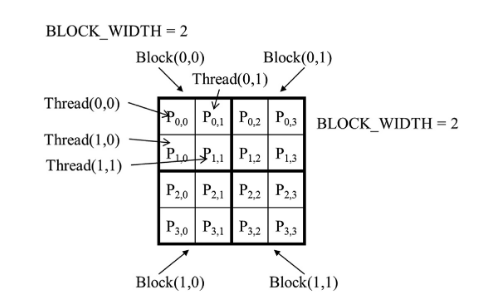
\includegraphics[width=\textwidth]{imgs/matrix_division.png}
        \caption{Divisione della matrice in una griglia di blocchi}
        \label{fig:1}
    \end{minipage}
    \hspace{0.05\textwidth}
    \begin{minipage}[b]{0.45\textwidth}
        \centering
        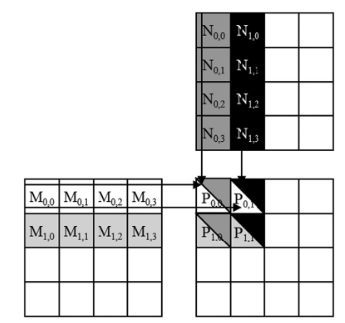
\includegraphics[width=\textwidth]{imgs/execution1.png}
        \caption{Esecuzione del kernel}
        \label{fig:2}
    \end{minipage}
\end{figure}

Questo è un approccio basilare con ampi margini di miglioramento. Infatti, in un contesto CUDA, è fondamentale ragionare tenendo in considerazione le prestazioni delle differenti memorie: la memoria globale è grande ma lenta, di controparte la memoria condivisa è piccola ma più veloce. Una strategia decisamente migliore rispetto a quella presentata in precedenza è quella di partizionare i dati in sottoinsiemi chiamati \textit{tiles}, in modo tale che ognuna di essa entri nella memoria condivisa con un importante vincolo: la computazione del kernel sulla singola tile può essere fatta indipendentemente dalle altre. Ad esempio, mostriamo gli accessi alla memoria globale che avvengono nella Figura~\ref{fig:2}:

\begin{figure}[H]
    \centering
    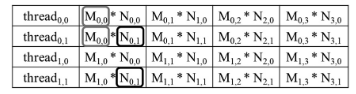
\includegraphics[width=0.6\textwidth]{imgs/memory_access.png}
    \caption{Accessi alla memoria globale}
    \label{fig:3}
\end{figure}

Nella Figura~\ref{fig:3} possiamo notare come gli stessi elementi vengano letti dalla lenta memoria globale in diversi step dell'esecuzione. In generale data la dimensione dei blocchi $width\times{width}$ ogni elemento delle matrici $\mathbf{A}$ e $\mathbf{B}$ è letto dalla memoria globale $width$ volte. L'idea è quindi quella di far collaborare i threads per caricare in memoria condivisa anticipatamente tutti i dati per poi procedere allo sviluppo dei calcoli cosi facendo stiamo riducendo di $\frac{1}{width}$ gli accessi alla memoria. La Figura~\ref{fig:4} mostra gli accessi alla memoria per questo approccio.

\begin{figure}[H]
    \centering
    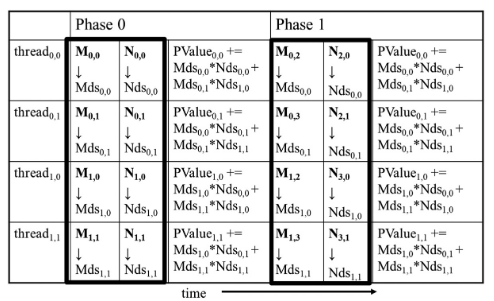
\includegraphics[width=0.6\textwidth]{imgs/memory_access1.png}
    \caption{Accessi alla memoria globale e caricamento in memoria condivisa}
    \label{fig:4}
\end{figure}

Il Listing~\ref{lst:2} mostra il kernel con l'approccio tiling e memoria condivisa.

\begin{lstlisting}[caption={Kernel CUDA con tiling e memoria condivisa}, label={lst:2}]
#define TILE_WIDTH 16
__global__ void matrixMulKernel(float* M, float* N, float* P, int Width) {
    __shared__ float Mds[TILE_WIDTH][TILE_WIDTH];
    __shared__ float Nds[TILE_WIDTH][TILE_WIDTH];

    int bx = blockIdx.x; int by = blockIdx.y;
    int tx = threadIdx.x; int ty = threadIdx.y;

    int Row = by * TILE_WIDTH + ty;
    int Col = bx * TILE_WIDTH + tx;

    float Pvalue = 0;
    for (int ph = 0; ph < Width/TILE_WIDTH; ++ph) {
        Mds[ty][tx] = M[Row*Width + ph*TILE_WIDTH + tx];
        Nds[ty][tx] = N[(ph*TILE_WIDTH + ty)*Width + Col];
        __syncthreads();

        for (int k = 0; k < TILE_WIDTH; ++k)
            Pvalue += Mds[ty][k] * Nds[k][tx];
        __syncthreads();
    }
    P[Row*Width + Col] = Pvalue;
}
\end{lstlisting}

\newpage

Il Listing~\ref{lst:2} nonostante ottimizzi l'uso delle memorie non funzionerebbe con matrici la cui $width$ non sia un multiplo di $TILE\_WIDTH$. Nel Listing~\ref{lst:3} è mostrata la soluzione approssimando per eccesso la divisione per $TILE\_WIDTH$ e riempendo con degli $0$ le parti di tile che non vanno effettivamente utilizzate:

\begin{lstlisting}[caption={Kernel CUDA con gestione dei bordi e tiling}, label={lst:3}]
float Pvalue = 0;
for (int ph = 0; ph < ceil(Width/(float)TILE_WIDTH); ++ph) {

    if ((Row < Width) && (ph*TILE_WIDTH+tx) < Width)
        Mds[ty][tx] = M[Row*Width + ph*TILE_WIDTH + tx];
    else
        Mds[ty][tx] = 0.0f;

    if ((ph*TILE_WIDTH+ty < Width) && (Col < Width))
        Nds[ty][tx] = N[(ph*TILE_WIDTH + ty)*Width + Col];
    else
        Nds[ty][tx] = 0.0f;

    __syncthreads();

    for (int k = 0; k < TILE_WIDTH; ++k)
        Pvalue += Mds[ty][k] * Nds[k][tx];

    __syncthreads();
}

if (Row < Width && Col < Width)
    P[Row*Width + Col] = Pvalue;
\end{lstlisting}

Il nostro scopo era quello di testare l'andamento delle prestazioni al variare del numero di thread e processi questo per quanto riguarda il kernel ne comporta l'adattamento in modo tale che un qualsiasi numero di thread (anche solo 1) possa effettuare in autonomia l'intero calcolo. Il Listing~\ref{lst:4} mostra questo adattamento con un grid-stride-loop. Si noti anche la definizione dinamica della memoria condivisa, in particolare viene usato 1 singolo array \textit{shared\_mem} la cui dimensione sarà uguale a $2\times{TILE\_WIDTH}\times{sizeof(double)}$ ovvero stiamo allocando lo spazio in memoria condivisa per salvare in modo contiguo nello stesso array le $2$ tile correnti da moltiplicare. Questo valore per assicurare le massime prestazioni dovrà essere $\leq cudaDevAttrMaxSharedMemoryPerBlock$ ovvero il limite hardware imposto dall'architettura della GPU che si sta usando.

\begin{lstlisting}[caption={Kernel CUDA generalizzato con tiling dinamico}, label={lst:4}]
__global__ void matrixMulKernel(double *A, double *B, double *C, int M, int N, int K) {
    extern __shared__ double shared_mem[];

    int tile_width = blockDim.x;

    double *s_A = (double *)shared_mem;
    double *s_B = (double *)shared_mem + tile_width * tile_width;

    int tx = threadIdx.x;
    int ty = threadIdx.y;

    int num_tiles_N = ceil((double)N / tile_width);
    int num_tiles_M = ceil((double)M / tile_width);
    int total_tiles = num_tiles_M * num_tiles_N;

    int block_id_1d = blockIdx.y * gridDim.x + blockIdx.x;
    int total_blocks = gridDim.x * gridDim.y;

    for (int tile_id = block_id_1d; tile_id < total_tiles; tile_id += total_blocks) {
        int by_tile = tile_id / num_tiles_N;
        int bx_tile = tile_id % num_tiles_N;

        int global_row = by_tile * tile_width + ty;
        int global_col = bx_tile * tile_width + tx;

        double c_value = 0.0;
        int phases = (K + tile_width - 1) / tile_width;

        for (int phase = 0; phase < phases; ++phase) {
            if ((global_row < M) && (phase * tile_width + tx < K))
                s_A[ty * tile_width + tx] = A[global_row * K + phase * tile_width + tx];
            else
                s_A[ty * tile_width + tx] = 0.0;

            if ((phase * tile_width + ty < K) && (global_col < N))
                s_B[ty * tile_width + tx] = B[(phase * tile_width + ty) * N + global_col];
            else
                s_B[ty * tile_width + tx] = 0.0;

            __syncthreads();

            for (int k = 0; k < tile_width; ++k)
                c_value += s_A[ty * tile_width + k] * s_B[k * tile_width + tx];

            __syncthreads();
        }

        if ((global_row < M) && (global_col < N))
            C[global_row * N + global_col] = c_value;
    }
}
\end{lstlisting}

\subsubsection{cuBLAS}
In alternativa a scrivere le proprie funzioni per il calcolo tra matrici, è disponibile la libreria cuBLAS sviluppata da NVIDIA che fornisce una versione ottimizzata per GPU delle routine BLAS (Basic Linear Algebra Subprograms), una serie standard di operazioni fondamentali in algebra lineare\footnote{\url{https://netlib.org/blas/}}. Sono inoltre disponibili diverse estensioni, tra cui cuBLASXt progettata per sfruttare più GPU contemporaneamente. Non sono necessari preparativi particolari, dato che si occupa autonomamente di allocare la memoria tra le GPU designate, distribuire il carico di lavoro tra di loro e infine recuperare i risultati sull'host\footnote{\url{https://docs.nvidia.com/cuda/cublas/index.html\#using-the-cublasxt-api}}.

Una nota tecnica riguarda la discrepanza tra l'ordine in memoria delle matrici: cuBLAS, per rimanere conforme alle specifiche Fortran di BLAS, si aspetta che i valori siano disposti per \textit{column-major} mentre lo standard nel linguaggio C/C++ è \textit{row-major}. Fortunatamente, è possibile evitare operazioni di memoria aggiuntive il fatto che i due metodi sono le rispettive trasposte e calcolare
$$
    \mathbf{C}^T=(\mathbf{B}\mathbf{A})^T
$$
Il risultato sarà quindi salvato in una matrice column-major e che quindi corrisponderà al risultato cercato leggendolo in row-major.

\section{Analisi}

\subsection{Ambiente di test}

TODO Pier: IBISCO

\subsection{Script e Configurazione dei Test}

Per gestire l'esecuzione di un vasto numero di test con configurazioni eterogenee, è stato implementato un processo automatizzato orchestrato dallo script \texttt{scripts/run.sh}. La sua esecuzione può essere suddivisa nelle seguenti fasi:

\begin{enumerate}
    \item \textbf{Inizializzazione e Pulizia:} La prima azione dello script è la preparazione dell'ambiente di esecuzione. Vengono rimossi i risultati di esecuzioni precedenti eliminando il contenuto delle directory \texttt{logs/ csv/ plots/ profiling/ bin/}, se in caso queste non dovessero esistere verranno create. Questo garantisce che ogni esecuzione parta da uno stato pulito e che i risultati non vengano contaminati da test precedenti.

    \item \textbf{Compilazione:} Viene compilato il codice sorgente presente nella directory \texttt{src/} usando \texttt{nvcc}. L'eseguibile risultante, \texttt{bin/main.out}, viene così aggiornato all'ultima versione del codice prima dell'avvio dei test.

    \item \textbf{Iterazione sui File di Configurazione:} Lo script itera su tutti i file con estensione \texttt{.csv} presenti nella directory \texttt{tests/}. Ciascun file definisce una famiglia di test; al suo interno, ogni riga (esclusa l'intestazione) specifica i parametri per una singola esecuzione.

    \item \textbf{Generazione e Sottomissione dei Job:} Per ogni riga di un file di configurazione, che rappresenta un singolo test, lo script esegue i seguenti passaggi:
          \begin{itemize}
              \item \textbf{Parsing dei Parametri:} I valori per \texttt{matrix\_size}, \texttt{n\_proc}, \texttt{n\_gpu}, \texttt{tile\_width}, \texttt{grid\_width} e \texttt{grid\_height} vengono estratti dalla riga corrente.
              \item \textbf{Creazione dello Script SLURM:} Viene generato dinamicamente uno script di sottomissione SLURM. Questo script contiene le direttive \texttt{\#SBATCH} necessarie per richiedere le risorse al cluster (nodi, task, GPU per task) e definire i file di output e di errore. Il comando di esecuzione principale è incapsulato da \texttt{nsys profile} per la profilazione, e l'eseguibile \texttt{bin/main.out} viene lanciato con i parametri specifici del test.
              \item \textbf{Sottomissione del Job:} Lo script SLURM appena creato viene sottomesso al gestore di code tramite il comando \texttt{sbatch}. L'ID del job restituito da SLURM viene catturato e memorizzato.
              \item \textbf{Gestione delle Dipendenze:} L'ID del job viene aggiunto a una lista di dipendenze che sarà utilizzata nella fase finale.
          \end{itemize}

    \item \textbf{Job di Analisi e Plotting:} Una volta che tutti i job di calcolo sono stati sottomessi, lo script genera un ultimo job SLURM. Questo job ha una dipendenza di tipo \texttt{afterok} da tutti i job sottomessi in precedenza. Ciò significa che verrà eseguito solo dopo che tutti i test di calcolo saranno terminati con successo. Il compito di questo job finale è eseguire lo script Python \texttt{scripts/plots.py}, che si occupa di aggregare i dati dai file \texttt{.csv} generati e di creare i grafici di performance.
\end{enumerate}

\subsection{Analisi delle misurazioni}
Purtroppo, a causa di problemi tecnici con la versione di OpenMPI presente sul cluster, non è stato possibile valutare in maniera significativa il programma. In particolare, la funzione usata per creare la griglia di processi\footnote{\url{https://docs.open-mpi.org/en/v5.0.x/man-openmpi/man3/MPI_Cart_create.3.html}} potrebbe fallire arbitrariamente causando la chiusura forzata dell'eseguibile. Sperimentazioni ausiliarie\footnote{\url{https://github.com/dev-shaa/mpi-test}} hanno portato eventualmente sempre allo stesso errore, il che fa presagire qualche problema in quella versione della libreria.

\subsection{NVIDIA Nsight Compute}

NVIDIA Nsight Compute è un profiler per CUDA che fornisce metriche dettagliate delle prestazioni e debug delle API tramite interfaccia utente e strumenti da riga di comando.
% TODO: che altro?

Purtroppo, a causa di problemi tecnici con il cluster, non è stato possibile valutare in maniera approfondita le metriche che sarebbero fornite da queste applicazioni.

\section{Esplorazione di NCCL}

\subsection{Introduzione}

\textbf{NVIDIA Collective Communications Library (NCCL)} è una libreria sviluppata da NVIDIA per facilitare operazioni di comunicazione collettiva ad alte prestazioni tra GPU, sia all'interno dello stesso nodo che su nodi distribuiti. NCCL fornisce primitive efficienti per operazioni come \texttt{broadcast}, \texttt{reduce}, \texttt{all-reduce}, \texttt{all-gather} e \texttt{reduce-scatter}, supportando pienamente ambienti multi-GPU e multi-nodo e sfruttando direttamente le interconnessioni ad alta velocità come NVLink, PCIe e InfiniBand.

L'architettura di NCCL è progettata per minimizzare la latenza e massimizzare il throughput delle comunicazioni tra GPU. Le sue caratteristiche principali includono:

\begin{itemize}
    \item \textbf{Topologia consapevole}: NCCL rileva automaticamente la topologia dell’hardware (PCIe, NVLink, InfiniBand) e costruisce percorsi di comunicazione ottimali.
    \item \textbf{Asincronicità}: Le operazioni sono progettate per essere non bloccanti e integrate nel flusso CUDA, permettendo una sovrapposizione efficiente tra comunicazione e computazione.
    \item \textbf{Comunicazione peer-to-peer}: Le GPU si scambiano direttamente i dati, evitando il passaggio attraverso la CPU e migliorando le prestazioni.
\end{itemize}

\subsection{API Principali}
Tra le principali API offerte da NCCL troviamo:
\begin{itemize}
    \item \texttt{ncclCommInitAll} / \texttt{ncclCommInitRank}: inizializzano i comunicatori per tutti i partecipanti al gruppo di comunicazione collettiva.
    \item \texttt{ncclBroadcast}: invia un buffer da una GPU a tutte le altre.
    \item \texttt{ncclAllReduce}: esegue una riduzione (es. somma) dei dati da tutte le GPU e distribuisce il risultato a tutte.
    \item \texttt{ncclReduceScatter}, \texttt{ncclAllGather}, \texttt{ncclReduce}, ecc.: altre primitive collettive standard.
    \item \texttt{ncclGroupStart} / \texttt{ncclGroupEnd}: permettono di raggruppare più operazioni per ottimizzarne l’esecuzione in pipeline.
\end{itemize}

Tutte queste operazioni lavorano direttamente su buffer residenti in memoria device (GPU) e possono essere lanciate su CUDA streams, permettendo un'esecuzione concorrente con il calcolo.

\subsection{Funzionamento}

\subsubsection{Throughput vs MPI}

NCCL è altamente ottimizzata per GPU moderne. In numerosi benchmark, NCCL ha dimostrato throughput superiori rispetto a implementazioni standard di MPI quando si tratta di comunicazioni intra-nodo tra GPU (specialmente via NVLink). Anche nel caso di multi-nodo, NCCL combinata con interconnessioni RDMA (come InfiniBand) può superare le prestazioni di MPI.

\subsubsection{Scalabilità}

La scalabilità è uno dei punti di forza principali:

\begin{itemize}
    \item Ottimizzato per architetture con decine o centinaia di GPU.
    \item Supporto trasparente per configurazioni eterogenee e distribuite.
    \item Adattamento automatico alla topologia hardware.
\end{itemize}

\subsubsection{Vantaggi su MPI}

L'interfaccia di NCCL è molto più semplice rispetto a quella di MPI, con un numero ridotto di funzioni ma fortemente specializzate. Questo rende più facile l’adozione, soprattutto per sviluppatori di applicazioni CUDA, a discapito però di una flessibilità inferiore: ne è un esempio la mancanza di tipi di dato complessi, topologie personalizzate, o comunicazioni puntuali.

\subsection{Svantaggi e Limitazioni}

Nonostante i vantaggi, NCCL presenta alcune limitazioni importanti:

\begin{itemize}
    \item \textbf{Overhead iniziale}: la creazione dei comunicatori nella fase iniziale dell'esecuzione può essere costosa, specialmente in ambienti distribuiti.
    \item \textbf{Meno flessibile di MPI}: NCCL non supporta comunicazioni punto-a-punto né tantomeno operazioni su topologie arbitrarie tra i processi.
    \item \textbf{Limitazioni hardware}: molte ottimizzazioni richiedono il supporto di NVLink o InfiniBand, non sempre presenti nei cluster generici. In assenza di queste il vantaggio in termini di prestazioni può essere ridotto o addirittura nullo.
    \item \textbf{Compatibilità}: la libreria è progettata esclusivamente per GPU NVIDIA e richiede versioni aggiornate del driver e dell’ambiente CUDA.
\end{itemize}

\subsection{Applicazione Potenziale all’Algoritmo SUMMA}

Nel contesto dell’algoritmo SUMMA, NCCL potrebbe essere utilizzata per ottimizzare le fasi di comunicazione collettiva.
L’idea alla base è sostituire le chiamate \texttt{MPI\_Bcast} per la propagazione dei pannelli delle matrici $\mathbf{A}$ e $\mathbf{B}$ lungo le righe e le colonne della griglia di processo, con due chiamate \texttt{ncclBroadcast} operate su due rispettivi comunicatori NCCL. In particolare:

\begin{itemize}
    \item Per ogni passo $k$, il pannello di $\mathbf{A}$ nella riga $i$ viene trasmesso a tutti i processi della riga tramite \texttt{ncclBroadcast}.
    \item Analogamente, il pannello di $\mathbf{B}$ nella colonna $j$ viene trasmesso a tutti i processi della colonna tramite un’altra \texttt{ncclBroadcast}.
\end{itemize}

Per implementare questa strategia sarebbe necessario creare due insiemi di comunicatori NCCL indipendenti, ciascuno rappresentante una delle due dimensioni della griglia logica di processi. L’utilizzo di \texttt{ncclGroupStart} e \texttt{ncclGroupEnd} consentirebbe l’accorpamento delle due comunicazioni in un’unica fase di sincronizzazione, migliorando ulteriormente l'efficienza.
Il codice risultante manterrebbe la stessa logica computazionale di SUMMA, ma con l'intento di sfruttare le ottimizzazioni hardware/software di NCCL nelle fasi di comunicazione collettiva.

Tuttavia, questa implementazione non è stata realizzata a causa della mancanza del supporto a NCCL nel cluster disponibile, rendendo non praticabile la sperimentazione.


\printbibliography

\end{document}
